\documentclass{beamer}
\usetheme{Madrid}
\usecolortheme{beaver}

\usepackage{tikz}
\usetikzlibrary{arrows.meta, positioning}

\begin{document}

\begin{frame}{Chaîne de traitement des données}
\centering
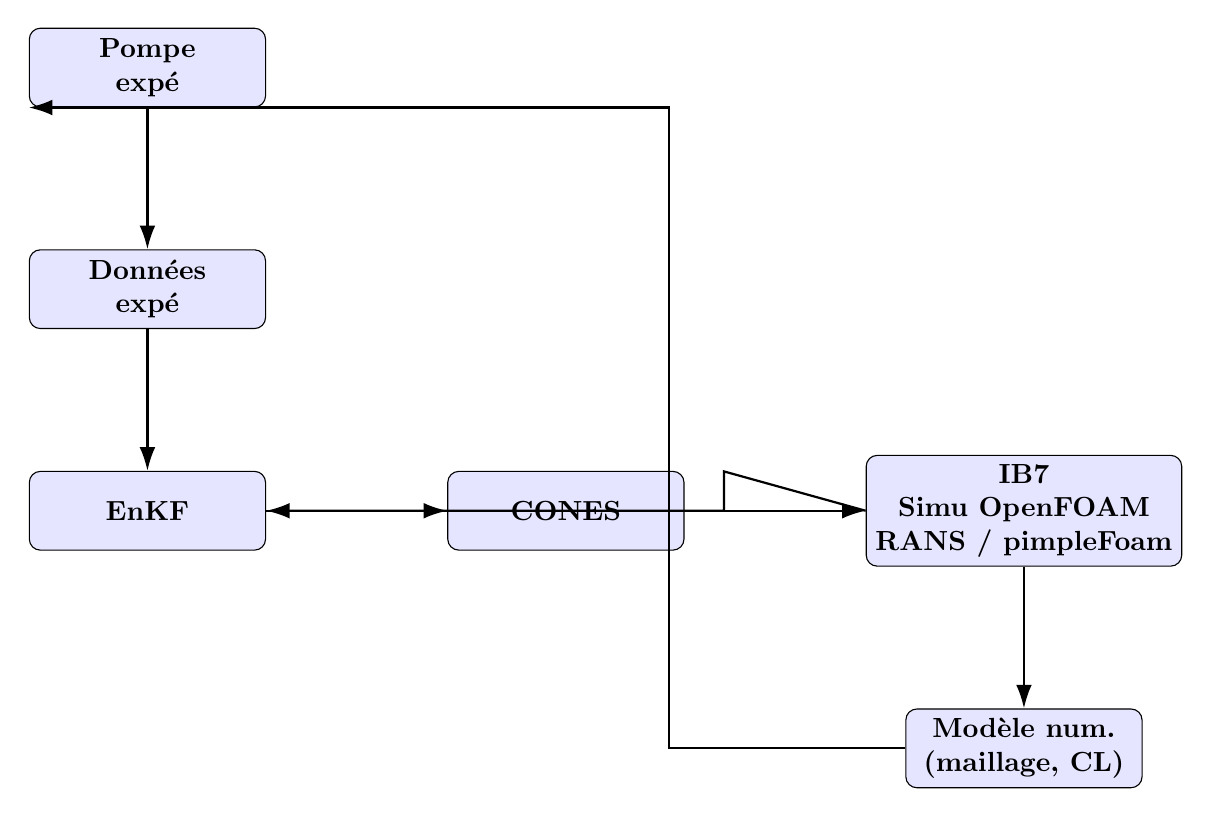
\begin{tikzpicture}[
    node distance=1.8cm and 2.3cm,
    box/.style={
        draw,
        rounded corners,
        minimum width=3cm,
        minimum height=1cm,
        align=center,
        font=\bfseries,
        fill=blue!10
    },
    arrow/.style={
        -{Latex[length=3mm,width=2mm]},
        thick
    }
]

% Nœuds
\node[box] (pump) {Pompe \\ expé};
\node[box, below=of pump] (data) {Données \\ expé};
\node[box, below=of data] (enkf) {EnKF};
\node[box, right=of enkf] (cones) {CONES};
\node[box, right=of cones] (ib7) {IB7 \\ Simu OpenFOAM \\ RANS / pimpleFoam};
\node[box, below=of ib7] (model) {Modèle num. \\ (maillage, CL)};

% Flèches principales
\draw[arrow] (pump) -- (data);
\draw[arrow] (data) -- (enkf);
\draw[arrow] (enkf) -- (cones);
\draw[arrow] (cones) -- (ib7);
\draw[arrow] (ib7) -- (model);

% Boucles
\draw[arrow] (model.west) -- ++(-3,0) |- (pump.south west);
\draw[arrow] (ib7.west) -- ++(-1.8,0.5) |- (enkf.east);

\end{tikzpicture}
\end{frame}

\end{document}
